\section{Phase 3}
In the third phase of this project, our goals were to flesh out pose detection for cars, and add in the ability to detect traffic light colors, and improve the rendering pipeline so that entire scenes could be rendered in a reasonable amount of time.

\subsection{Improved Depth Detection}
Another issue which presented itself in previous phases was the issue with using the centroid of the bounding box for depth estimation. Objects could be occluded in a such a way that the centroid lay on pixels which did not actually belong to the object, and as such the depth would be predicted incorrectly. To solve this, the segmentation version of YOLOv9 was used, which provided a mask for each bounding box of a detected object. A simple scheme wherein the median of the depth of each pixel in the mask was used as the depth of the object was implemented. The difference between the outputs of the two network versions, as well as the resulting depth mask, is shown in Figure \ref{fig:depth}.

\begin{figure}
  \centering
  \begin{subfigure}{0.9\linewidth}
    \centering
    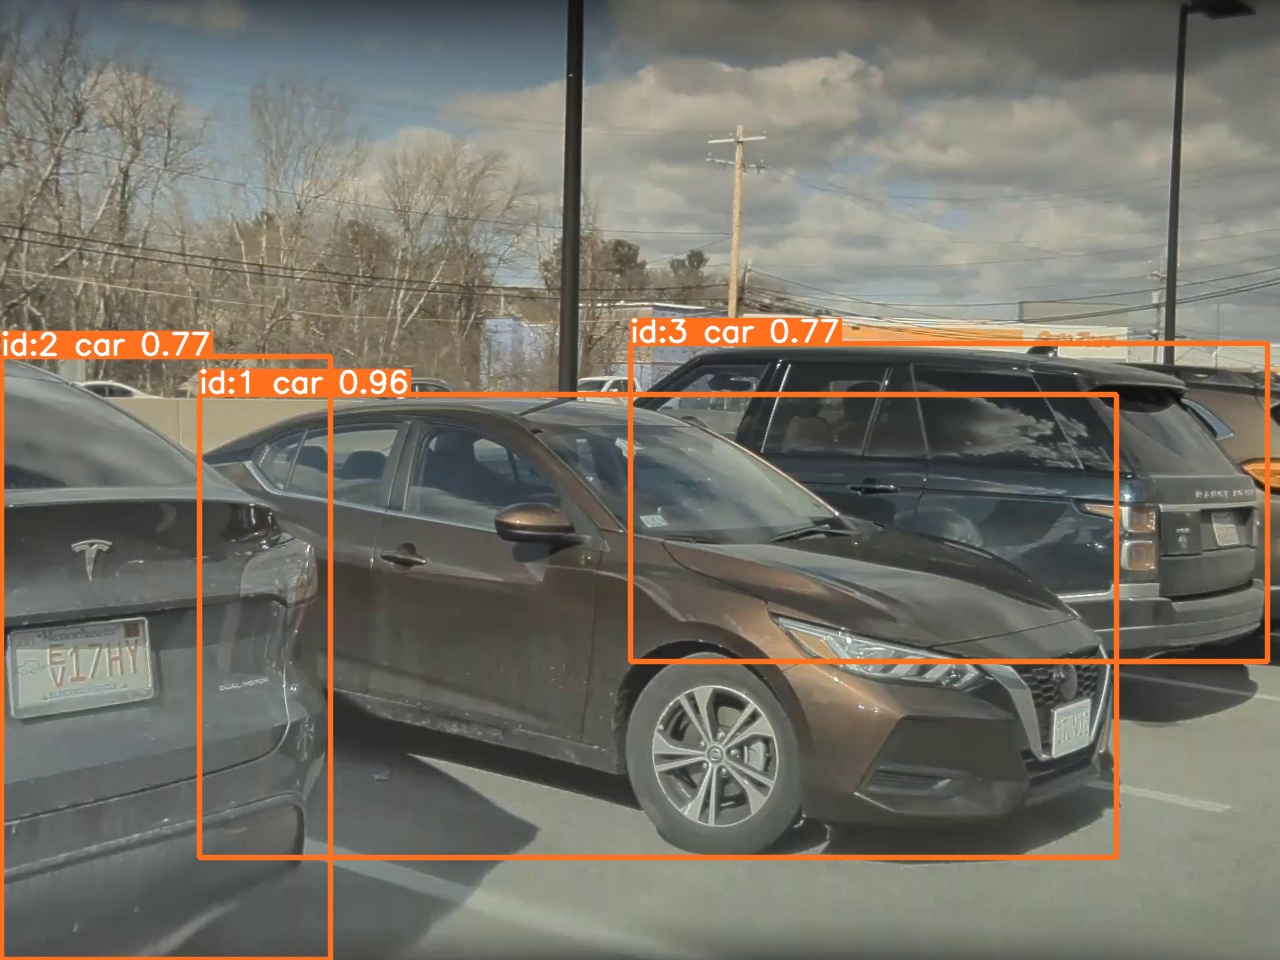
\includegraphics[width=0.95\textwidth]{images/YOLOv9_without_seg.jpg}
    \caption{YOLOv9 without segmentation.}
  \end{subfigure}
  \begin{subfigure}{0.9\linewidth}
    \centering
    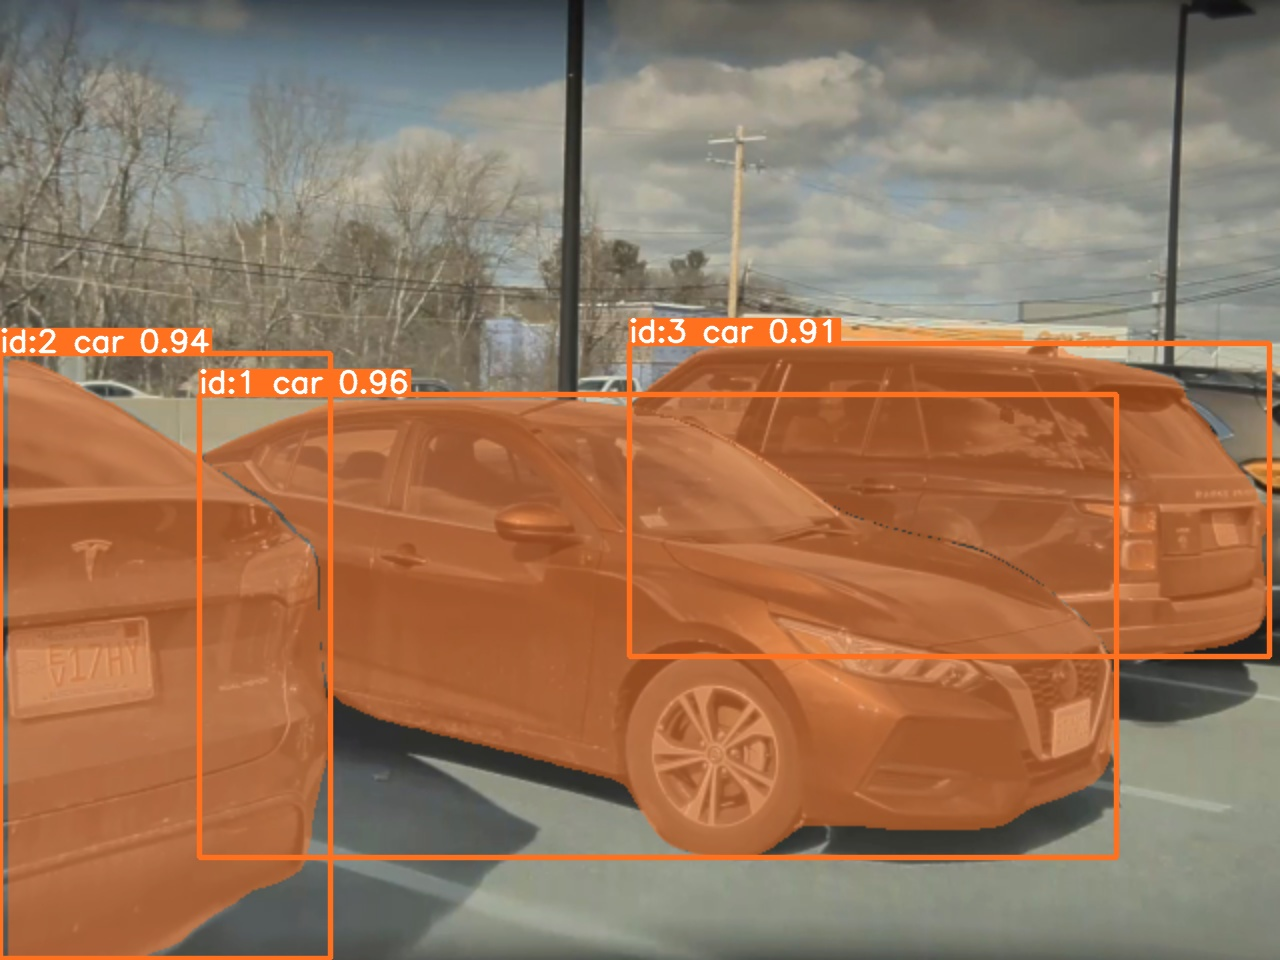
\includegraphics[width=0.95\textwidth]{images/YOLOv9_with_seg.jpg}
    \caption{YOLOv9 with segmentation.}
  \end{subfigure}
  \begin{subfigure}{0.9\linewidth}
    \centering
    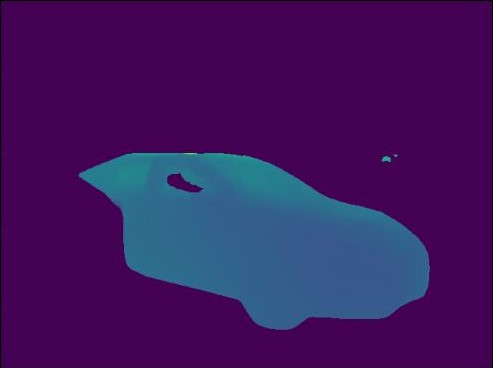
\includegraphics[width=0.95\textwidth]{images/masked_depth.jpg}
    \caption{Masked depth of one car. Notice the outlier points, which are ignored using the median scheme.}
  \end{subfigure}
  \caption{Improved depth detection using segmentation.}
  \label{fig:depth}
\end{figure}

Another consideration with the depth estimation, as mentioned in Phase 1, is the fact that the ZoeDepth estimates the depth of the object's surface. This was accounted for partially by offsetting the depth of detected vehicles by one meter.

\subsection{Improved Lane Detection}
When running the CLRNet pipeline on some test videos, the output proved very poor, and so causes of the poor performance were assessed. First, hyperparameters of the network were tuned, specifically the cut distance, image size, and sampling range parameters, but these did not lead to consistently better results. Our team then noticed that the pre-trained weights and configuration of the network were set up for the CULane dataset, which did not match our input data well. The network also had weights and configuration for the LLAMAS dataset, which matched our input data much better, and so the hyperparameters were transferred to the existing LLAMAS configuration, and the network was tested again. This time, the output was significantly better, as shown in Figure \ref{fig:lane_detection}.

\begin{figure}
  \centering
  \begin{subfigure}{0.9\linewidth}
    \centering
    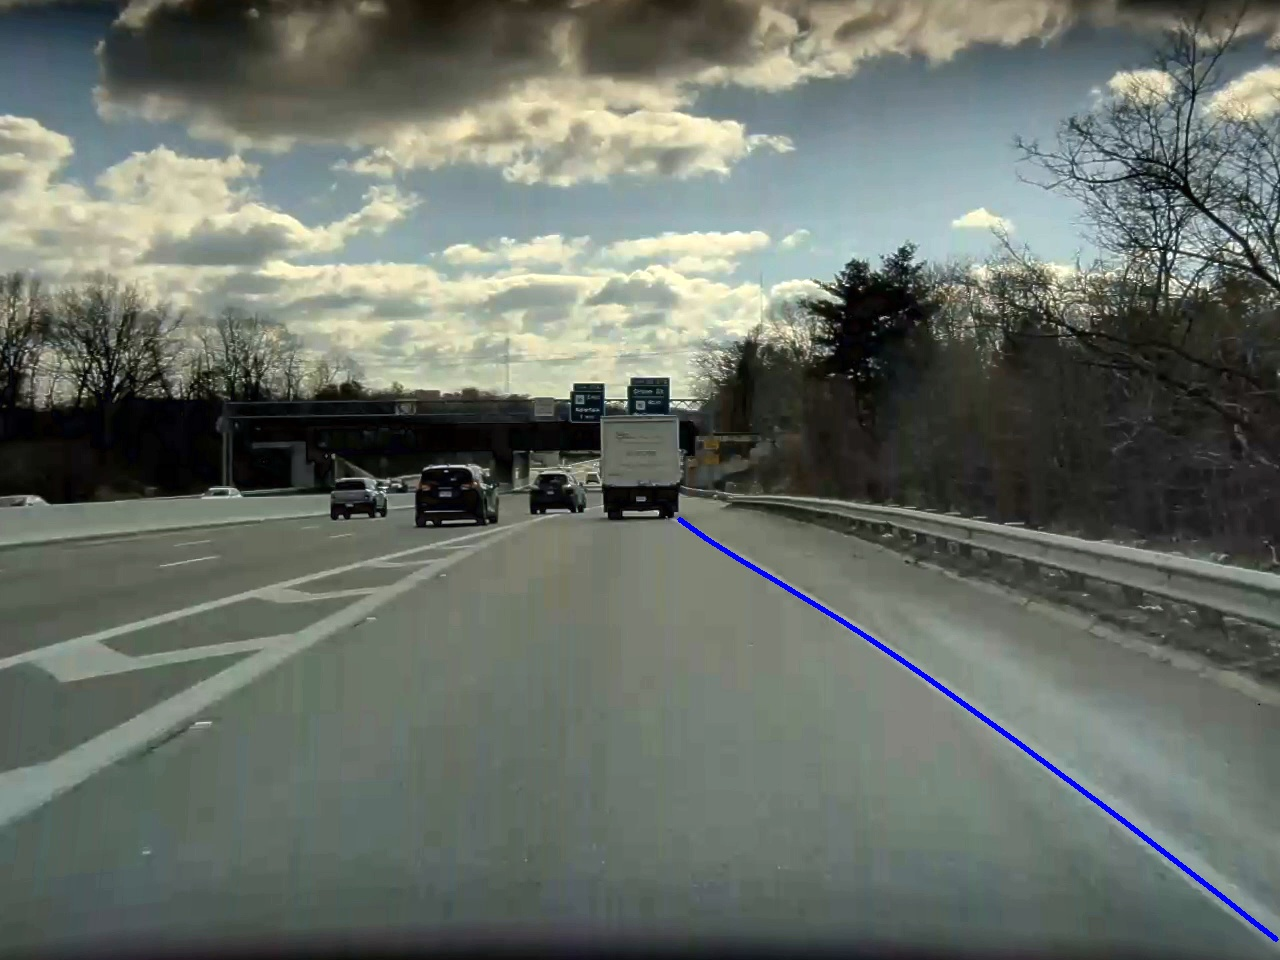
\includegraphics[width=0.95\textwidth]{images/lanes_culane.jpg}
    \caption{CULane weights and configuration.}
  \end{subfigure}
  \begin{subfigure}{0.9\linewidth}
    \centering
    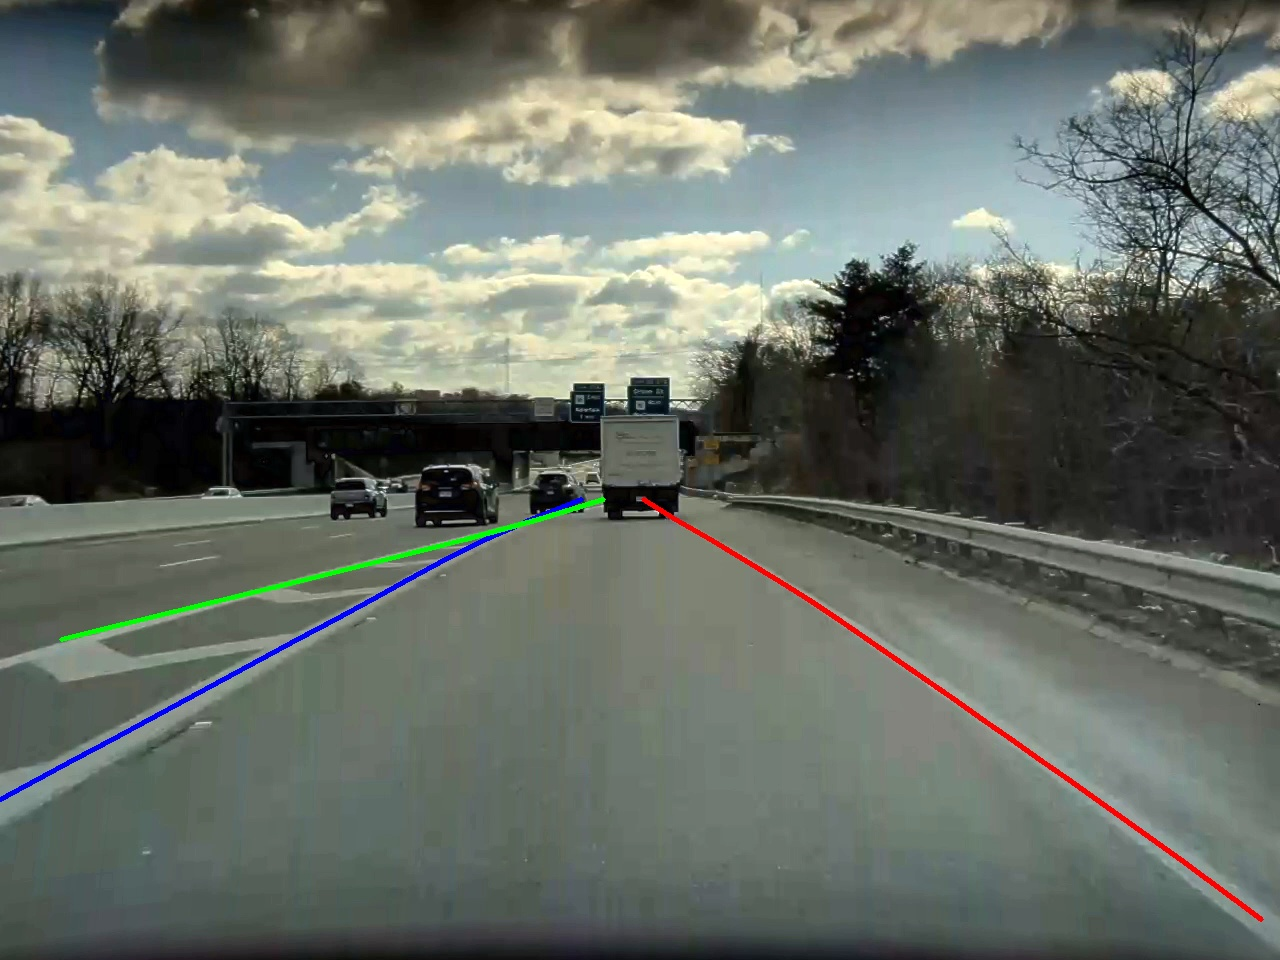
\includegraphics[width=0.95\textwidth]{images/lanes_llamas.jpg}
    \caption{LLAMAS weights and configuration.}
  \end{subfigure}
  \caption{Comparison of CLRNet lane detection on a difficult frame using two different weights and configurations.}
  \label{fig:lane_detection}
\end{figure}

\subsection{Pedestrian Pose Estimation}
Pedestrian pose estimation was performed using derivative of YOLOv8 trained on poses, provided by Ultralytics \cite{YOLOv8Pose}. This network detected pedestrians and accurately predicted poses, but we were unable to integrate it into our pipeline. The output of the network is shown in Figure \ref{fig:pedestrian_pose}.

\begin{figure}
  \centering
  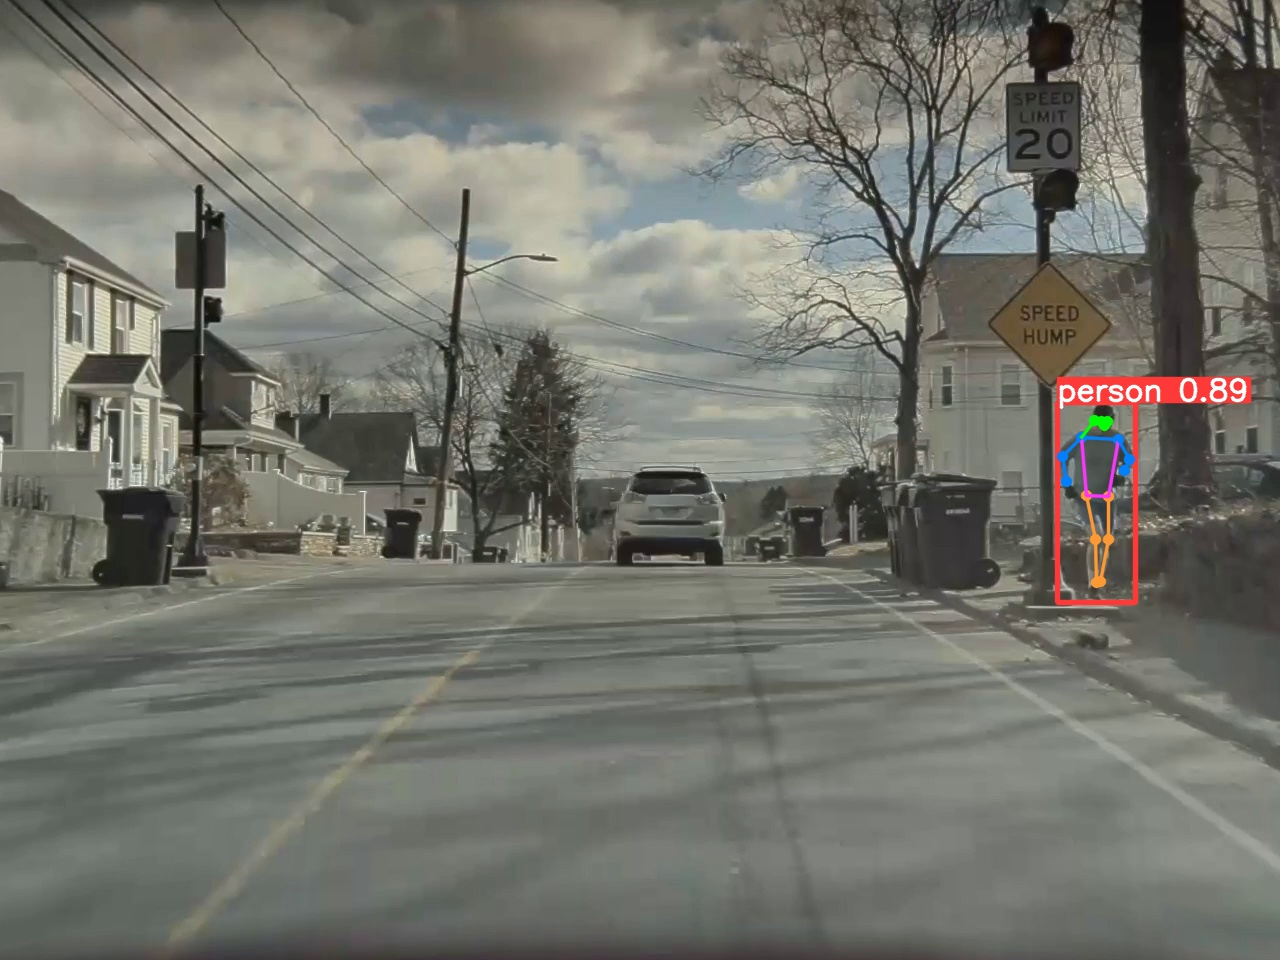
\includegraphics[width=0.95\linewidth]{images/pedestrian_pose.jpg}
  \caption{Pedestrian pose estimation using YOLOv8.}
  \label{fig:pedestrian_pose}
\end{figure}

\subsection{Improved Rendering Pipeline}
The pipeline for rendering an entire scene was also improved in this stage. The details of the rendering pipeline are shown in Figure \ref{fig:pipeline} in Appendix \ref{app:pipeline}.

\section{Shortcomings}
After completing our entire pipeline, there are clearly some shortcomings, and things our team could simply not get working. Most notably car pose estimation and traffic light color detection were not fully implemented. There were some other subtle things missing, such as traffic cones, rigging pedestrian model in blender, lane type, speed limit signs, break light detection, and moving vs stationary vehicles. Most of these features were not implemented as networks found for the task could not be made to function on our data, but others were simply not implemented due to time constraints.

Of the pipelines our team did get working, the biggest limitations were the use of 2D lane line estimation, and the lack of robust 3D orientation information for detected objects.